%%%%%%%%%%%%%%%%%%%%%%%%%%%%%%%%%%%%%%%%%%%%%%%%
% E.Pinault-Bigeard - e.pinault-bigeard@upsti.fr
% http://s2i.pinault-bigeard.com
% CC BY-NC-SA 2.0 FR - http://creativecommons.org/licenses/by-nc-sa/2.0/fr/
%%%%%%%%%%%%%%%%%%%%%%%%%%%%%%%%%%%%%%%%%%%%%%%%
\documentclass[11pt]{article}
%%%%%%%%%%%%%%%%%%%%%%%%%%%%%%%%%%%%%%%%%%%%%%%%
% Package UPSTI_Document
%%%%%%%%%%%%%%%%%%%%%%%%%%%%%%%%%%%%%%%%%%%%%%%%

\usepackage{import}
%
%%%%%%%%%%%%%%%%%%%%%%%%%%%%%%%%%%%%%%%%%%%%%%%%
% Package UPSTI_Document
%%%%%%%%%%%%%%%%%%%%%%%%%%%%%%%%%%%%%%%%%%%%%%%%
\usepackage{subcaption}
\usepackage[usenames, svgnames, dvipsnames]{xcolor}
\usepackage{UPSTI_Document}
\usepackage{pgfplots}
\usepackage{import}
\definecolor{darkspringgreen}{rgb}{0.09, 0.45, 0.27}

\newcommandx*{\dessinRepereFigGeo}[5][1=\vx{},2=\vy{},3=\vz{},4=,5=0]
	{
		\draw [->,very thick] (0,0) -- (1,0) ;
		\draw [->,very thick] (0,0) -- (0,1) ;
    \fill[white] (0,0) circle (0.13);
    \draw [->,very thick] (0,0) circle (0.13);
    \ifnumequal{#5}{0} {% z vers nous
      \fill[black] (0,0) circle (0.03);
      \draw [->,thick] (0,0) circle (0.04);
    }{% z vers la feuille
  		\begin{scope} [rotate=45]
  			\draw [-,thick] (0,-0.12) -- (0,0.12) ;
  			\draw [-,thick] (-0.12,0) -- (0.12,0) ;
  		\end{scope}
    }
		\draw [anchor=north west] (1.1,0) node {${#1}$};
		\draw [anchor=south west] (0,1.1) node {${#2}$};
		\draw [anchor=north east] (-0.1,0) node {${#3}$};
		\draw [anchor=north west] (-0.1,-0.1) node {${#4}$};
	}

	\usepackage{array}
	\newcolumntype{L}[1]{>{\raggedright\let\newline\\\arraybackslash\hspace{0pt}}m{#1}}
	\newcolumntype{C}[1]{>{\centering\let\newline\\\arraybackslash\hspace{0pt}}m{#1}}
	\newcolumntype{R}[1]{>{\raggedleft\let\newline\\\arraybackslash\hspace{0pt}}m{#1}}

	\usepackage{pifont}% http://ctan.org/pkg/pifont
\newcommand{\cmark}{\color{green}\ding{51}}%
\newcommand{\xmark}{\color{red}\ding{55}}%
\newcommand{\fmark}{\ding{229}}%
\newcommand{\itemc}{\item[\cmark]}%
\newcommand{\itemx}{\item[\xmark]}%
\newcommand{\itemf}{\item[\fmark]}%

\usepackage{tikz-timing}
\usepackage{circuitikz}
%---------------------------------%
% Paramètres du package
%---------------------------------%

% Version du document (pour la compilation)
% 1: Document prof
% 2: Document élève
% 3: Document à publier
\newcommand{\UPSTIidVersionDocument}{2}

% Classe
% 1: PTSI				6: PSI*			11: TSI2		16: Spé
% 2: PT	(par défaut)	7: MPSI			12: ATS
% 3: PT*				8: MP			13: PC
% 4: PCSI				9: MP*			14: PC*
% 5: PSI				10: TSI1		15: Sup
%\newcommand{\UPSTIidClasse}{2}



% Matière
% 1: S2I (par défaut)    2: IPT     3: TIPE
% 6: Vie au lycée
\newcommand{\UPSTIvariante}{5}
\newcommand{\UPSTIidMatiere}{0}
\newcommand{\UPSTIintituleMatiere}{Automatique}
\newcommand{\UPSTIsigleMatiere}{Autom}
% Type de document
% 0: Custom*				7: Fiche Métho de			14: Document Réponses
% 1: Cours (par défaut)		8: Fiche Synthèse    		15: Programme de colle
% 2: TD     				9: Formulaire
% 3: TP						10: Memo
% 4: Colle					11: Dossier Technique
% 5: DS						12: Dossier Ressource
% 6: DM						13: Concours Blanc
% * Si on met la valeur 0, il faut décommenter la ligne suivante:
%\newcommand{\UPSTItypeDocument}{Custom}
\newcommand{\UPSTIidTypeDocument}{1}

% Titre dans l'en-tête


% Titre dans l'en-tête

\newcommand{\UPSTIvariante}{5}

\newcommand{\UPSTItitreEnTete}{Automatisme industriel}
%\newcommand{\UPSTItitreEnTetePages}{}
\newcommand{\UPSTIsousTitreEnTete}{Introduction aux API}


% Titre
%\newcommand{\UPSTItitrePreambule}{Automatisme industriel}
\newcommand{\UPSTItitre}{La programmation d'un Automate Industriel}

% Durée de l'activité (pour DS, DM et TP)
\newcommand{\UPSTIduree}{3h30}

% Note de bas de première page
%\newcommand{\UPSTInoteBasDePremierePage}{Geoffrey Vaquette}
% Numéro (ajoute " n°1" après DS ou DM)
\newcommand{\UPSTInumero}{2}

% Numéro chapitre
%\newcommand{\UPSTInumeroChapitre}{1}

% En-tête customisé
%\newcommand{\UPSTIenTetePrincipalCustom}{UPSTIenTetePrincipalCustom}

% Message sous le titre
%\newcommand{\UPSTImessage}{Message sous le titre}


% Référence au programme
%\newcommand{\UPSTIprogramme}{\EPBComp \EPBCompP{B1-02}, \EPBCompP{B2-49}, \EPBCompS{B2-50}, \EPBCompS{B2-51}, \EPBCompP{C1-07}, \EPBCompP{C1-08}}

% Si l'auteur n'est pas l'auteur par défaut
%\renewcommand{\UPSTIauteur}{WWOOOOOOWW}

% Si le document est réalisé au nom de l'équipe
%\newcommand{\UPSTIdocumentCollegial}{1}

% Source
\newcommand{\UPSTIsource}{G. Vaquette, H. Discours}

% Version du document
\newcommand{\UPSTInumeroVersion}{0.3}

%-----------------------------------------------
\UPSTIcompileVars		% "Compile" les variables
%%%%%%%%%%%%%%%%%%%%%%%%%%%%%%%%%%%%%%%%%%%%%%%%


% Titre
%\newcommand{\UPSTItitrePreambule}{Automatisme industriel}
\newcommand{\UPSTItitre}{Cablâge des entrée d'un API simple} 
\usetikzlibrary{arrows,automata,circuits.plc.ladder}

\newlength{\ladderskip}
\setlength{\ladderskip}{5\tikzcircuitssizeunit} % 5\tikzcircuitssizeunit = 35pt
\newlength{\ladderrungsep}
\setlength{\ladderrungsep}{.2\ladderskip}
\def\ladderrungend#1{\pgftransformyshift{-#1\ladderskip-\ladderrungsep}}

\ctikzset{
	logic ports=ieee,
	logic ports/scale=0.7,
}



\newcommand{\automaintienMachineEtat}[0]{
\begin{tikzpicture}[->,>=stealth',shorten >=1pt,auto,node distance=3cm,
                    semithick]
  %\tikzstyle{every state}=[fill=none,draw=none,text=white]

  \node[initial,state] (A)              {M1};
  \node[state]         (B) [right of=A] {M2};

  \path (A) edge [bend left]  node {$B_pM$} (B)
        (B) edge [bend left]  node {$B_pA$} (A);
\end{tikzpicture}
}


%%%%%%%%%%%%%%%%%%%%%%%%%%%%%%%%%%%%%%%%%%%%%%%%
% Début du document
%%%%%%%%%%%%%%%%%%%%%%%%%%%%%%%%%%%%%%%%%%%%%%%%
\begin{document}
\UPSTIbuildPage

%\UPSTIobjectif{Durant cette activité, nous allons analyser une trame pour l'envoi d'informations sur une étiquette.}

\tableofcontents
\pagebreak

Du point de vue d'un automate, les modules d'entrées ont pour objectif l'acquisition d'information en provenance des capteurs. Ces informations peuvent être de type logique, analogique ou numérique. 

\section{Introduction}
Chaque type de module permet d'acquérir un certain type d'information. Par exemple, un module d'entrées logique permettra d'acquérir l'état d'un capteur logique. Il ne pourra pas interpréter les informations en provenance d'un capteur analogique. 

Afin de permettre l'interprétation des données par le programme, ces dernières sont stoquées dans la mémoire de l'automate. On pourra alors accéder à l'état des entrées en associant une variable à la case mémoire correspondant à cette entrée. 

Dans ce cours, nous n'adresserons que le cas simple des automates Logo. 


\section{Entrées logiques}
\subsection{Les capteurs logiques}
\subsubsection{Les capteurs passifs}
Un capteur passif et un capteur ne nécéssitant pas d'alimentation pour fonctionner, c'est le cas, entre autres, d'un interrupteur, d'un bouton poussoir ou encore d'un capteur fin de course. 

Un tel capteur comporte deux fils et laissera passer le signal d'un fil à l'autre s'il est \textbf{fermé} ou coupera le signal s'il est \textbf{ouvert}. Il existe en existe deux types : normalement fermé ou normalement ouvert. 

Pour chacun de ces capteur, il existe une version normalement ouvert (\textbf{NO} \textit{Normaly Open}) et une version normalement fermée (\textbf{NC} \textit{Normaly Closed}). 

La figure~\ref{fig:captPassif} représente quelques exemples de capteurs passifs. 

\begin{figure}[h]
	\centering
	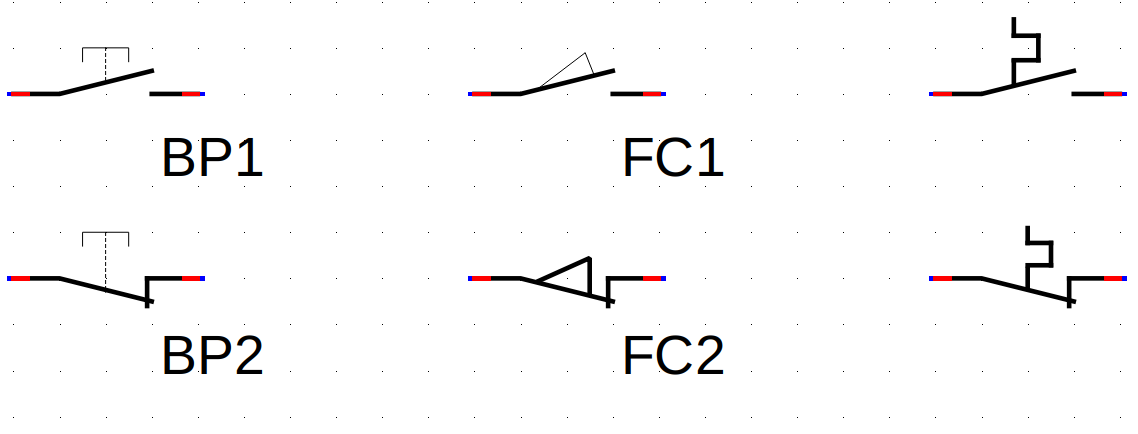
\includegraphics[width=.8\textwidth]{images/capteurPassifs.png}
	\caption{Capteurs passifs}
	\label{fig:captPassif}
\end{figure}


\subsubsection{Les capteurs actifs}
	Les capteurs actifs sont des capteurs nécessitant une alimentation pour fonctionner, c'est le cas, entre autres, d'un capteur de proximité inductif ou capacitif, d'un capteur infrarouge, etc. 

	Un tel capteur comporte trois fil. Deux d'entre-eux servent à alimenter le capteur et le dernier délivre le signal logique correspondant à son état. 

	Ils peuvent être représenté sous la forme d'une boite à trois fils ou d'un interrupteur associé à un symboôle spécifique. La figure~\ref{fig:captActif} représente un capteur inductif et un capteur capacitif PNP (compatible avec le logo). 
\begin{figure}
	\centering
	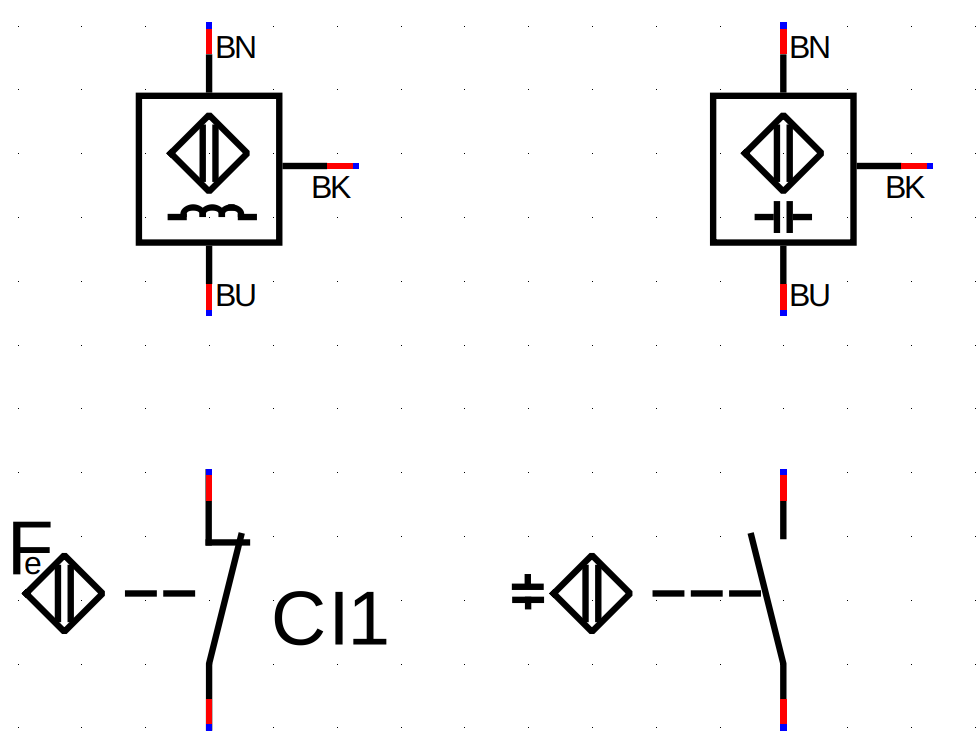
\includegraphics[width=.4\textwidth]{images/captActifs.png}
	\caption{Capteurs actif - 3 fils}
	\label{fig:captActif}
\end{figure}

\subsection{Le module d'entrées logiques}
Puisqu'un capteur logique délivre une information \textit{Tout ou Rien} , il peut être représenté sous la forme d'un interrupteur quelque soit le type du capteur utilisé. 


\subsubsection{Technologie}
Une interface d'entrée logique est composée de 
\begin{itemize}
	\item Bornes d'entrées
	\begin{itemize}
		\item Une borne pour chaque entrée
		\item Un point commun à toutes les entrées
	\end{itemize}
	\item Une isolation galvanique
	\item Un circuit d'acquisition
\end{itemize}

Sur les Logo que nous utilisons, la borne commune est reliée en interne à la masse (on dit que les entrées sont de type \textit{SINK}, nous verrons ce que cela signifie ultérieurement). La figure~\ref{fig:entreeLogo} schématise le fonctionnement d'une entrée logique sur un automate. Notons que dans le cas présent, le courant entre par la borne d'entrée et ressort par le point commun, la masse. 

\begin{figure}
	\centering
	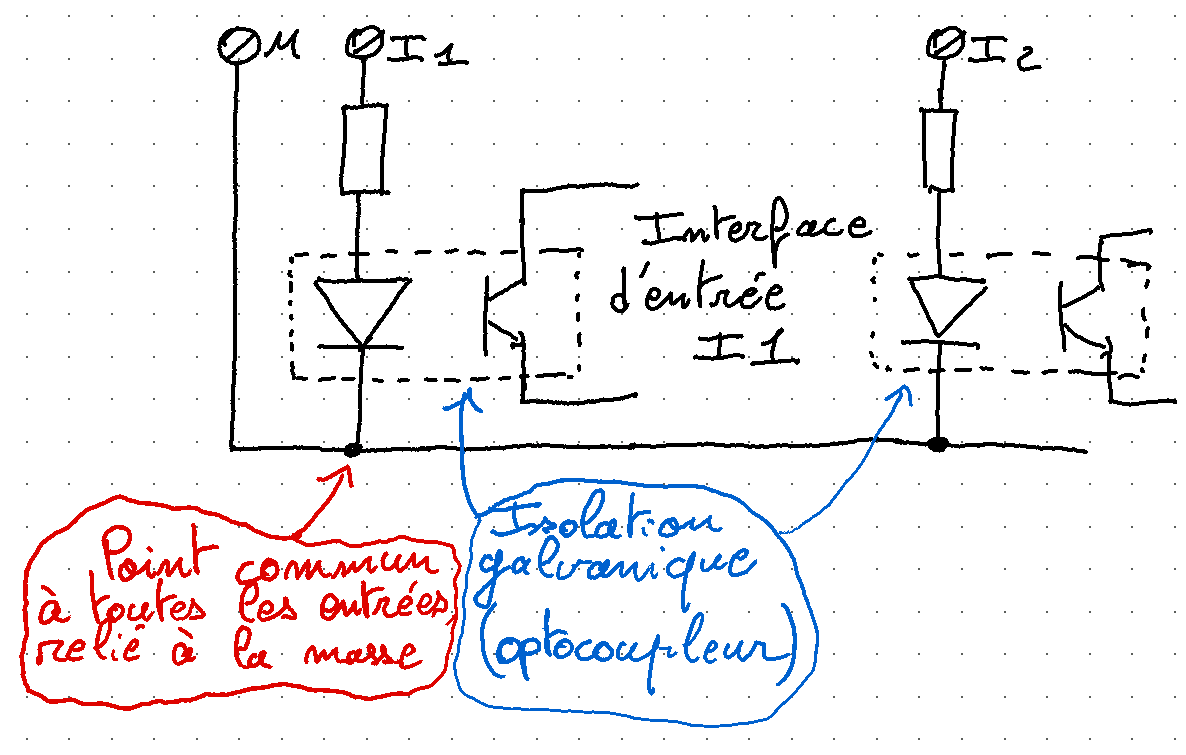
\includegraphics[width=.8\textwidth]{images/C04-interneLogo.png}
	\caption{Interface d'entrée logique d'un LOGO}
	\label{fig:entreeLogo}
\end{figure}
\pagebreak
\subsection{Cablâge}
\begin{UPSTIactivite}
	\UPSTIquestion{Compléter la figure suivante en cablant les différents capteurs logiques}
	\begin{center}
		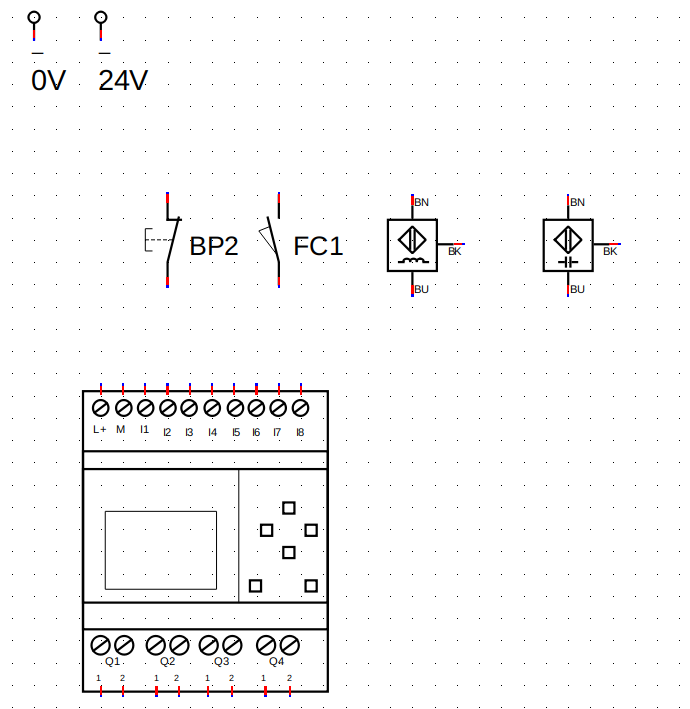
\includegraphics[width=.6\textwidth]{images/C04-aCompleter.png}
	\end{center}
\end{UPSTIactivite}

\section{Entrées analogiques}
Pour interpréter et exploiter des capteurs délivrant une information analogique comme la température, l'humidité, la pression, etc. il est nécessaire de récupérer et de stoquer l'information dans la mémoire de l'automate. 

Il existe des modules spécialisés dans l'acquisition de ce type d'information, qui font l'objet de cette section. 

\subsection{Conversion Analogique Numérique (CAN)}
Supposons un capteur délivrant une \textbf{tension} image d'une grandeur (température par exemple). Cette tension sera convertie en une valeur numérique via un \textbf{Convertisseur Analogique Numérique (CAN)}. Ce dernier fera la traduction d'une tension comprise dans sa plage de fonctionnement en une valeur binaire codées sur $n$ bits. 

\UPSTIaRetenir{
	Un \textbf{C}onvertisseur \textbf{A}nalogique \textbf{N}umérique convertie une tension comprise dans sa plage de fonctionnement en un nombre binaire codé sur $n$ bits. 
	\begin{description}
		\item[Plage de fonctionnement : ]Tensions minimale et maximale de la traduction analogique -> numérique
		\item[Résolution : ]Nombre de bits sur lequel est codée la valeur traduite
	\end{description}
}

\begin{figure}[h]
	\centering
	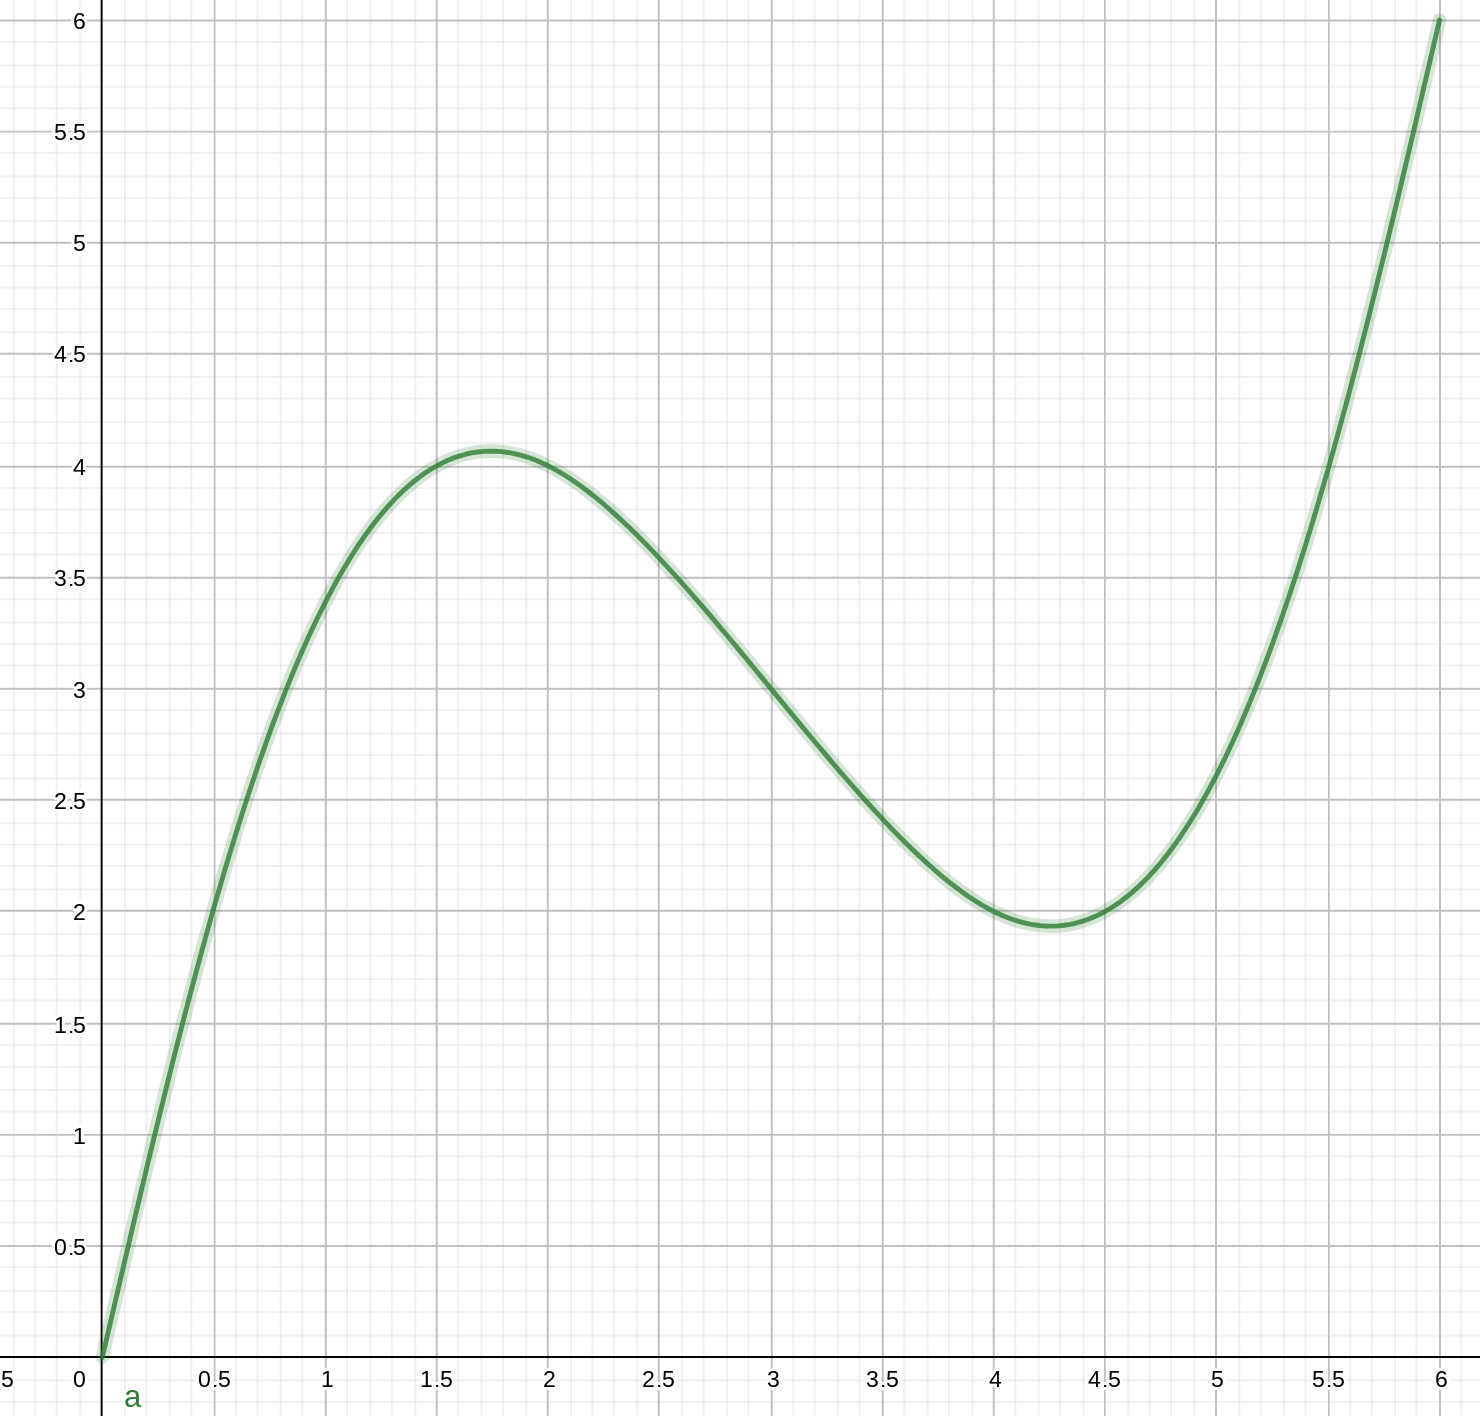
\includegraphics[width=.6\textwidth]{images/courbeAutom.png}
	\caption{Traduction d'un signal selon deux résolutions différentes}
	\label{fig:signalCAN}
\end{figure}

\begin{UPSTIactivite}
	\UPSTIquestion{Sur la Figure~\ref{fig:signalCAN}, représenter le signal sous une forme numérique codée sur 4 bits.}
\end{UPSTIactivite}
\subsection{Câblage d'un capteur analogique délivrant une tension sur un LOGO}
Cette section prend à nouveau l'exemple simple d'un Logo. 
Sur le module de base, les entrées 7 et 8 sont utilisables en entrée analogique \textbf{0-10 V}. Il est donc possible d'utiliser un capteur analogique délivrant une tension sur cette plage directement sur ces entrées. La tension est mesurée entre le potentiel de l'entrée en question et la masse. 

\begin{UPSTIactivite}
	\UPSTIquestion{Dessiner le cablâge d'un capteur de température délivrant un signal sur 0-10V sur l'entrée I8 d'un automate LOGO}
	\UPSTIquestion{Dessiner le cablâge d'un potentiometre \SI{15}{k\ohm} alimenté par une alimentation 12V}
	\vspace{7cm}
\end{UPSTIactivite}

\subsection{Câblage d'un capteur analogique délivrant une tension sur un LOGO}
Certains modules sont spécialisés pour l'interprétation de données en provenance d'un capteur délivrant un courant. Là encore, une plage est définie. 

Cependant, le module de base du LOGO ne comporte que deux entrées analogiques Pour un capteur délivrant un courant au lieu d'une tension, il est alors indispensable de convertir le courant délivré par le capteur en une tension compatible (et le plus adapté possible) avec la plage de fonctionnement du CAN utilisé. 
La façon la plus simple de réaliser cette conversion est l'utlisation d'une résistance \textbf{judicieusement choisie}
\pagebreak
\begin{UPSTIactivite}
	\UPSTIquestion{Dessiner le cablâge d'un capteur de luminosité délivrant un courant compris entre 0 et \SI{50}{mA} sur l'entrée I8 d'un automate LOGO}
	\vspace{7cm}
\end{UPSTIactivite}


\end{document}
